% Copyright (C) 2011,2012,2013,2014,2015,2016 The ESPResSo project
%  
% This file is part of ESPResSo.
%   
% ESPResSo is free software: you can redistribute it and/or modify it
% under the terms of the GNU General Public License as published by the
% Free Software Foundation, either version 3 of the License, or (at your
% option) any later version.
%  
% ESPResSo is distributed in the hope that it will be useful, but
% WITHOUT ANY WARRANTY; without even the implied warranty of
% MERCHANTABILITY or FITNESS FOR A PARTICULAR PURPOSE.  See the GNU
% General Public License for more details.
%  
% You should have received a copy of the GNU General Public License
% along with this program.  If not, see <http://www.gnu.org/licenses/>.
%
\documentclass[
a4paper,                        % paper size
11pt,                           % font size
twoside,                        % two sided
footsepline,                    % add a line to separate the footer
headsepline,                    % add a line to separate the header
headexclude,                    % header does not belong to the text
footexclude,                    % footer does not belong to the text
pagesize,                       % set the pagesize in a DVI document
bibtotocnumbered,               % add the bibliography to the TOC
idxtotoc                        % add the index to the TOC
%openright,                      % start a new chapter on the right page
%,DIV12
%,draft
]{scrreprt}

\usepackage[draft]{varioref}    % defines \vref
\usepackage{hyperref}           % automatically creates links when
                                % using pdflatex, defines \url
\usepackage{ifpdf}              % defines \ifpdf
\usepackage{graphicx}           % handles graphics
\usepackage{makeidx}            % creates the index
\usepackage{color}              % use colors

\usepackage{amsmath}

\usepackage{calc}               % compute length
\usepackage{ifthen}             % provide ifthen
\usepackage{xspace}
\usepackage{units}
\usepackage[numbers]{natbib}

% For building the distribution docs, disable todo boxes.
%\usepackage[disable]{todonotes}
\usepackage{todonotes}

%%%%%%%%%%%%%%%%%%%%%%%%%%%%%%%%%%%%%%%%%%%%%%%%%%
%%%%%%%%%%%%%%%%%%%%%%%%%%%%%%%%%%%%%%%%%%%%%%%%%%
%%%%%%%%% New Commands and Environments %%%%%%%%%%
%%%%%%%%%%%%%%%%%%%%%%%%%%%%%%%%%%%%%%%%%%%%%%%%%%
%%%%%%%%%%%%%%%%%%%%%%%%%%%%%%%%%%%%%%%%%%%%%%%%%%
\newcommand{\es}{\mbox{\textsf{ESPResSo}}\xspace}
\newcommand{\ie}{\textit{i.e.}\xspace}
\newcommand{\eg}{\textit{e.g.}\xspace}
\newcommand{\etal}{\textit{et al.}\xspace}


%%%%%%%%%%%%%%%%%%%%%%%%%%%%%%%%%%%%%%%%%%%%%%%%%%
%%%%%%%%%%%%%%%%%%%%%%%%%%%%%%%%%%%%%%%%%%%%%%%%%%
%%%%%%%%%%%%%%%% Other Settings %%%%%%%%%%%%%%%%%%
%%%%%%%%%%%%%%%%%%%%%%%%%%%%%%%%%%%%%%%%%%%%%%%%%%
%%%%%%%%%%%%%%%%%%%%%%%%%%%%%%%%%%%%%%%%%%%%%%%%%%
\makeindex

%%%%%%%%%%%%%%%%%%%%%%%%%%%%%%%%%%%%%%%%%%%%%%%%%%
%%%%%%%%%%%%%%%%%%%%%%%%%%%%%%%%%%%%%%%%%%%%%%%%%%
%%%%%%%%%%%%%%%%% Main Document %%%%%%%%%%%%%%%%%%
%%%%%%%%%%%%%%%%%%%%%%%%%%%%%%%%%%%%%%%%%%%%%%%%%%
%%%%%%%%%%%%%%%%%%%%%%%%%%%%%%%%%%%%%%%%%%%%%%%%%%
\begin{document}
\titlehead{
  \begin{center}
    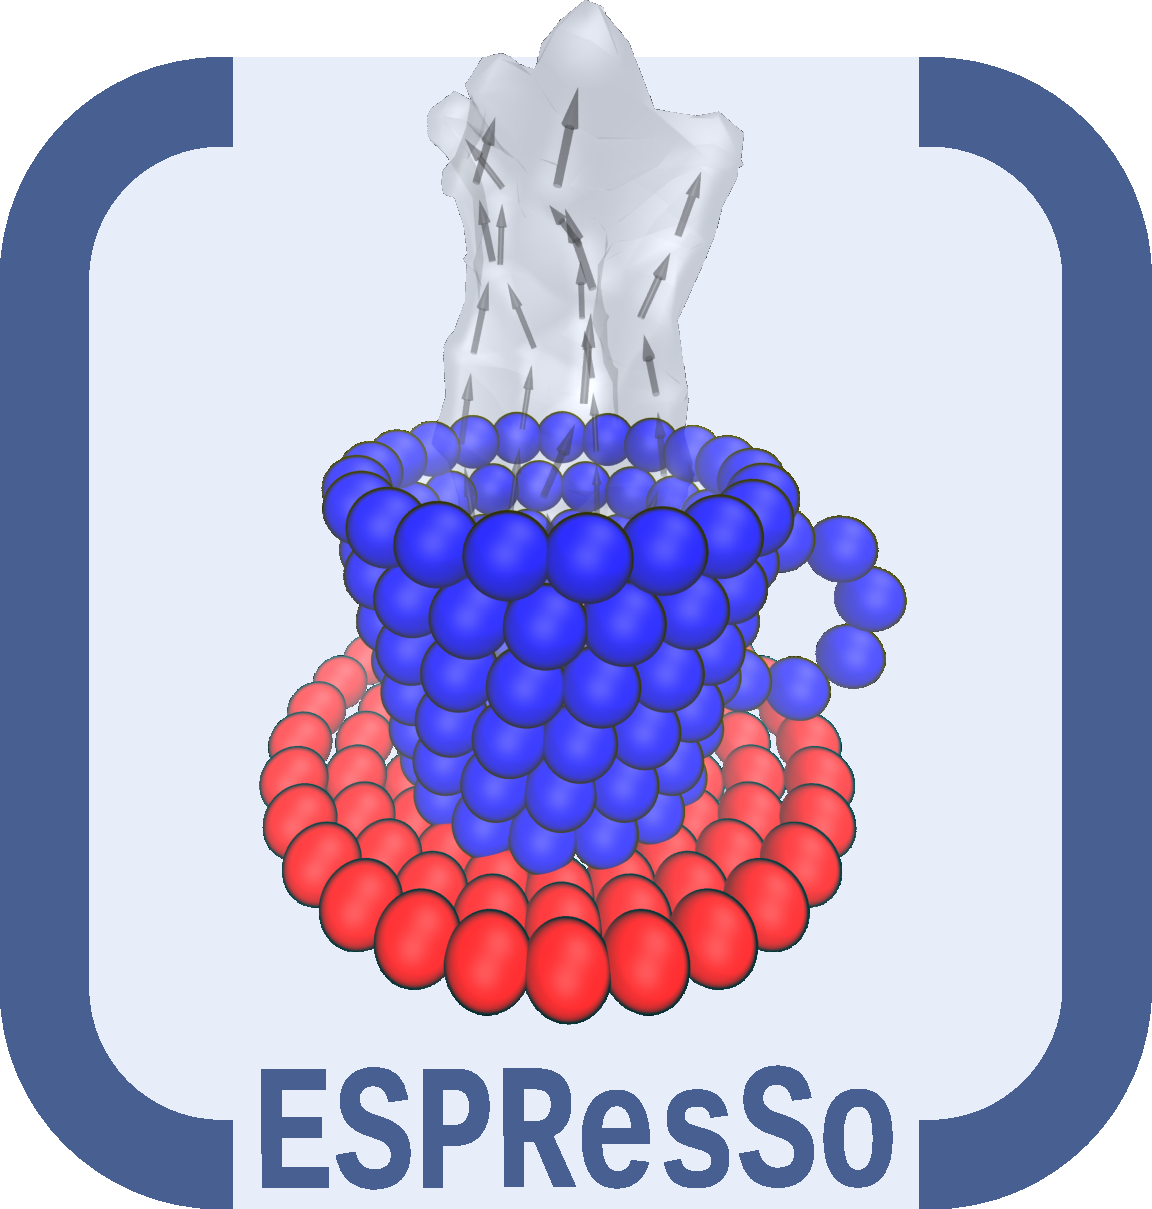
\includegraphics[width=5cm]{logo/logo.pdf}
  \end{center}
}
\title{\es Developer's Guide}
\date{\today}
\ifdefined\esversion%
\author{for version \esversion}
\fi%

\maketitle

\tableofcontents

\chapter{Getting into Contact}

The first thing that you should do when you want to start to
participate is to get into contact with the \es developers. To do
that, subscribe to the developers' mailing list at
\url{http://lists.nongnu.org/mailman/listinfo/espressomd-devel} and
write a short email to the list address
\texttt{espressomd-devel@nongnu.org} where you state your experience
with simulations and programming and the things that you would like to
do in \es. We do not bite, and we are happy about anybody who wants to
participate!

\chapter{Development Environment}
\label{sec:env}

\section{Required Development Tools}
\label{sec:requirements}

If you want to participate in the development of \es, you will require
the following tools depending on what tasks you want to perform:

\begin{itemize}
\item To be able to access the development version of \es, you will
  need the distributed versioning control system
  Git\footnote{\url{http://git-scm.com/}}.  Section \vref{sec:git}
  contains documentation on how we employ git.
\item To build \es from the development sources, you will need not too
  old versions of the ``GNU autotools'' (\ie
  automake\footnote{\url{http://www.gnu.org/software/automake/}} and
  autoconf\footnote{\url{http://www.gnu.org/software/autoconf/autoconf.html}})
  installed on your system. Section \vref{sec:build_devel} contains
  information on how to build the development code, section
  \vref{sec:build_system} contains details on how the build system
  works.
\item To be able to compile the User's Guide or the Developer's Guide,
  you will need a \LaTeX-installation (all recent ones will do). For
  details, refer to chapter \vref{sec:docs}.
\item To compile the Doxygen code documentation, you will need to have
  the tool \textsc{Doxygen}\footnote{\url{http://www.doxygen.org/}}.
\end{itemize}

All of these tools should be easy to install on most Unix operating
systems.

\section{Building the Development Code}
\label{sec:build_devel}

\begin{itemize}
\item Use \texttt{bootstrap.sh} before building the code.
\item Use configure with \texttt{--enable-maintainer-mode}.
\item Possible targets of \texttt{make}
  \begin{itemize}
  \item \texttt{check}
  \item \texttt{dist}
  \item \texttt{doc}
  \item \texttt{ug}
  \item \texttt{dg}
  \item \texttt{doxygen}
  \item \texttt{tutorials}
  \item \texttt{distcheck}
  \item \texttt{clean}, \texttt{distclean}
  \end{itemize}
\end{itemize}


\section{Git Repositories}
\label{sec:git}

\begin{itemize}
\item Development Repository: \url{https://github.com/espressomd/espresso}
\item 

Code hosting at GNU Savannah
  \url{https://savannah.nongnu.org/projects/espressomd/}

\end{itemize}
\section{Jenkins Build Server}
\label{sec:jenkins}

\url{http://espressomd.org/jenkins}
\begin{itemize}
\item \es homepage \url{http://espressomd.org}
\item Jenkins build server 
\end{itemize}

\section{Build System}
\label{sec:build_system}

The build system of \es makes use of the GNU autotools suite
consisting of
automake\footnote{\url{http://www.gnu.org/software/automake/}} and
autoconf\footnote{\url{http://www.gnu.org/software/autoconf/autoconf.html}}.
If you want to use the development source code of ESPResSo, you first
need to install both of these tools.

The central source files of the build system are the following:
\begin{itemize}
\item \texttt{configure.ac}
\item \texttt{config/*.m4}
\item \texttt{Makefile.am}
\item the different \texttt{Makefile.am} in the subdirectories
\end{itemize}

To change the behaviour of the build system, you have to modify any
these files.

\subsection{Running \texttt{bootstrap.sh}}

The script \texttt{bootstrap.sh} in the top level source directory can
be used to run \texttt{automake}, \texttt{autoconf} and the associated
tools to generate the \texttt{configure} script and the
\texttt{Makefile.in} used during compilation.  Once
\texttt{bootstrap.sh}, the \es development code can be build and used
like the release code.

\subsection{Creating a Distribution Package}

As described in the User's Guide, to create a \texttt{.tar.gz}
distribution file that contains all required files, you can simply run
\texttt{make dist}. This will bundle all files and put them into an
archive with the name
\texttt{espresso-\textit{version}\texttt{.tar.gz}}.

Even better, you can also run \texttt{make distcheck}. This will not
only create the distribution file, but it will also thoroughly check
the created distribution, \ie it will try to 
\begin{itemize}
\item unpack the distro into a new directory
\item configure and build it (\texttt{configure})
\item run the testsuite (\texttt{make check})
\item install it into a new directory (\texttt{make install})
\item uninstall it (\texttt{make uninstall})
\end{itemize}
Whenever something goes wrong in these checks, it will give an error
message that describes the problem. When everything goes fine, you can
be relatively sure that you have a useful \es distribution
package.

In some cases, it might be necessary to pass some options to the run
of \texttt{configure} done by \texttt{make distcheck}>. To these ends,
the environment variable \texttt{DISTCHECK\_CONFIGURE\_FLAGS} can be
set to the required options.

\paragraph{Example}
\begin{verbatim}
DISTCHECK_CONFIGURE_FLAGS="--without-mpi CPPFLAGS=\"-I /usr/include/tcl8.4\"" \
  make distcheck
\end{verbatim}

\subsection{Adding New Files}

To add new files to \es (like C source files or header files)
you need to do the following:
\begin{itemize}
\item Add the files to the \texttt{Makefile.am} in the same directory
\item Run \texttt{bootstrap.sh} in the source directory
\item Check the distribution by using \verb!make distcheck!
\item Add the files to the Git repository
\end{itemize}

\section{Testsuite}
\label{sec:testsuite}

\begin{itemize}
\item How to write tests?
\item How they are called (\texttt{runtest.sh})
\end{itemize}

\chapter{Documentation}

\section{User's Guide}

The User's Guide is written in \LaTeX. The source files reside in the
subdirectory \texttt{doc/ug/} of the \es sources. The master file is
\texttt{ug.tex}, each chapter is contained in its own source file.

\subsection{General issues}

\begin{itemize}
\item Other than usual, in the UG's \texttt{.tex}-files, the
  underscore character ``\_'' is a normal character in most cases, \ie
  it can be used unquoted. Unfortunately, however, this makes it
  impossible to use ``\_'' in \LaTeX-labels (don't ask me why!).
\item Headings should start with a capital letter and continue with
  lower-case letters (``First steps'' and \emph{not} ``First Steps'').
\item Use the ``-ing'' form in headings, \ie ``Setting up particles''
  instead of ``Particle setup'' or the like.
\item To see which parts of the User's guide need to be fixed or which
  documentation is missing, there is a \verb!\todo!-command where one
  can put notes about what remains to be done. In the release version,
  the boxes are disabled so that they do not disturb the users. They
  can be turned on by commenting out the appropriate line in
  \texttt{ug.tex}:
\begin{verbatim}
%% For building the distribution docs, disable todo boxes.
%\usepackage[disable]{todonotes}
\usepackage{todonotes}
\end{verbatim}

\end{itemize}

\subsection{Building the User's Guide}
\begin{itemize}
\item To build the User's Guide, you need to have a \LaTeX-installation
  that includes BibTeX, PDFLaTeX and makeindex. All installations that
  I know of provide these tools.
\item There are two methods to build the User's Guide:
  \begin{itemize}
  \item Use \texttt{make ug} from the build directory to build
    it. This will automatically generate the \es quick reference
    and call latex, bibtex and makeindex as required.
  \item Use \texttt{perl latexmk} from the source directory. This will
    basically do the same, however, it will \emph{not} automatically
    update the quick reference. The advantage of this method is, that
    you can use all of \texttt{latexmk}'s nice features, such as
    \texttt{-pvc}. You can always rebuild the quick reference manually
    by calling 
    \begin{verbatim}
awk -f assemble_quickref.awk > quickref.inp
    \end{verbatim}
  \end{itemize}
\end{itemize}

\subsection{Adding New Files}

To add new \LaTeX-files to the User's Guide, you need to modify
\begin{itemize}
\item \texttt{ug.tex}: add an appropriate include command near the end
  of the file
\item \texttt{Makefile.am}: add the file to the variable
  \texttt{ug\_TEXFILES}. 
\end{itemize}

\subsection{Additional Environments and Commands}

To maintain a consistent layout, a number of environments and
commands have been defined that should be used where applicable. 
\begin{itemize}
\item For the description of \es's Tcl-commands, read \ref{tcl_docs}.
\item The name of \es should be set via the command \verb!\es!.
\item The strings ``\ie'', ``\eg'' and ``\etal'' should be set via
  \verb!\ie!, \verb!\eg! and \verb!\etal!.
\item For short pieces of code that can be displayed inline, use
  \verb!\codebox{!\textit{text}\verb!}! or \verb|\verb!|\textit{text}\verb|!|
\item For longer code pieces or the syntax decription of non-Tcl
  commands, the environment \texttt{code} exists:
\begin{verbatim}
\begin{code}
  ...
\end{code}
\end{verbatim}
  Note that this is \emph{not} a verbatim environment, \ie it will
  evaluate \LaTeX-commands that are used inside. Therefore, the
  characters \verb!\!, \verb!{! and \verb!}! need to be quoted with
  backslashes inside the environment!  Also, the underscore character
  ``\_'' needs to be quoted like \verb!\_!. On the other hand, it is
  possible to use other layout commands (like \verb!\textit!) inside.
\item For pieces of Tcl-code that make extensive use of \verb!{! and
    \verb!}!, a verbatim environment \verb!tclcode! exists: 
\begin{verbatim}
\begin{tclcode}
 ...
\end{tclcode}
\end{verbatim}
\end{itemize}

\subsection{Documentation of Tcl commands}
\label{tcl_docs}

\subsubsection{Formal Syntax Definition}

All \es-commands have to be documented in the User's Guide.

The command
\verb!\newescommand[!\textit{label}\verb!]{!\textit{command}\verb!}!
should be used at the beginning of a command description to generate a
label \verb!es:!\textit{command} and create appropriate index
entries. The optional argument \textit{label} is only required, when
\textit{command} contains an underscore character ``\_''. In that
case, a label \verb!es:!\textit{label} is generated that should not
contain an underscore character.

For the \emph{formal syntax definition}, you have to use the
environments \texttt{essyntax} or \texttt{essyntax*}.  Both will
generate the headings \emph{Syntax} and
\emph{Description}. \texttt{essyntax} will furthermore copy the syntax
definition to the quick reference guide.  For an example, look at the
documentation of the \texttt{part} command in the file
\texttt{part.tex}. Inside the \texttt{essyntax} environment, you have
to use the following commands for typesetting the definition:
\begin{itemize}
\item \verb!\variant{!\textit{number}\verb!}! to typeset the label of a
  command variant
\item \verb!\var{!\textit{name}\verb!}! to typeset a variable
  argument. Note, that the argument is typeset in math mode.  This
  means, that you can use ``\_'' to denote a subscript.
\item \verb!\keyword{!\textit{text}\verb!}! or
  \verb!\lit{!\textit{text}\verb!}! to typeset keywords or literals.
\item \verb!\opt{!\textit{text}\verb!}! to typeset optional
  arguments. Note that usually, the text inside the \texttt{opt}
  command will not be wrapped. If the optional argument is pretty long
  and needs to be wrapped, use \verb!\optlong!.
\item \verb!\optlong{!\textit{text}\verb!}! to typeset long optional
  argument blocks.
\item \verb!\alt{!\textit{alt1} \verb!\asep! \textit{alt2}
    \verb!\asep! \textit{alt3} \dots \verb!}! to typeset alternatives.
\item \verb!\feature{!\textit{feature}\verb!}! to typeset when a
  \textit{feature} is referred to.
\item \verb!\require{!\textit{number}\verb!}{!\textit{text}\verb!}! to
  typeset \textit{text} to show that it requires certain features of
  \es. \textit{number} denotes the marking that is shown next to
  \textit{text}. When this command is used, you also have to use the
  \texttt{features}-environment (see below) at the end of the
  \texttt{essyntax} environment, where all of the \textit{number}s
  used are explained.
\item The environment \texttt{features} to typeset which features are
  required by the Tcl-command. Inside the environment, each feature
  should be declared via the command
  \verb!\required[!\textit{number}\verb!]{!\textit{feature}\verb!}!,
  where the optional argument \textit{number} is the number used above
  and \textit{feature} is the feature in capital letters.
\end{itemize}

The formal syntax definition should be as simple and as readable as
possible, as it will be what a user references to. Avoid very long
definitions and constructs like nested alternatives and options.  In
those cases, prefer to split the syntax definition into several
variants instead of writing it in a single, complicated definition.

\paragraph{Example}
\begin{verbatim}
\begin{essyntax}
[clip]
\variant{5} constraint pore 
  center \var{c_x} \var{c_y} \var{c_z} 
  axis \var{n_x} \var{n_y} \var{n_z} 
  radius \var{rad}
  length \var{length} 
  type \var{id} 

\require{1}{%
  \variant{6} constraint rod center \var{c_x} \var{c_y} 
  lambda \var{lambda}
} 
  
\require{1}{%
  \variant{7} constraint plate height \var{h}
  sigma \var{sigma} 
}
  
\require{2,3}{%
  \variant{8} constraint ext_magn_field \var{f_x} \var{f_y} \var{f_z} 
}

  \begin{features}
  \required{CONSTRAINTS}
  \required[1]{ELECTROSTATICS}
  \required[2]{ROTATION}
  \required[3]{DIPOLES}
  \end{features}
\end{essyntax}
\end{verbatim}

\subsubsection{Description}

In the description, you should use all of the above typesetting
commands when you refer to them in the text.  In particular, every
variable argument introduced via the \verb!\var!-command in the
definition has to be explained in detail:
\begin{itemize}
\item state explicitly the \emph{type} of the argument (integer,
  float, string, Tcl-list)
\item explain the meaning of the argument
\end{itemize}

If the command has a number of different options, \ie independent,
optional arguments, they can be described in the \emph{arguments}
environment:
\begin{verbatim}
\begin{arguments}
  \item[<arg1>] <description of arg1>
  \item[<arg2>] <description of arg2>
  ...
\end{arguments}
\end{verbatim}

The environment will generate the subheading \emph{Arguments} and
nicely format the descriptions.

\paragraph{Example}
\begin{verbatim}
\begin{arguments}
  \item[\opt{\alt{short \asep verbose}}] Specify, whether the output is
    in a human-readable, but somewhat longer format (\keyword{verbose}),
    or in a more compact form (\keyword{short}). The default is
    \keyword{verbose}.
  
  \item[\opt{\alt{folded \asep absolute}}] Specify whether the particle
    positions are written in absolute coordinates (\keyword{absolute})
    or folded into the central image of a periodic system
    (\keyword{folded}). The default is \keyword{absolute}.
  
  ...
\end{arguments}
\end{verbatim}

\section{Doxygen Code Documentation}
\label{sec:doxygen}

The documentation of each function should contain a short description,
if necessary a more detailed description and a description for the
return value and parameters.

Look at the documentation of existing files and functions to get a
feeling how it should be!

Doxygen is able to understand simple \LaTeX\ and HTML commands as well
as some special command in order to give the documentation a nice
structure and to make it more readable. In the following list you find
a short description of the most common commands we need:

\begin{itemize}
\item \verb!\anchor! \textit{name} \textit{description}\\
  Create an anchor to which you can refer using the \verb!\ref!
  command.
\item \verb!\ref! \textit{name} \texttt{["}\textit{text}\texttt{"]}\\
  Insert a link to another object in the documentation (\eg an
  anchor).
\item \verb!<a href="http://www.your_url.html">title</a>!\\
  Link to an external HTML source.
\item \verb!\file! \textit{name} \textit{description}\\
  Special anchor for a file.
\item \verb!\image html! \textit{image}\\
  Include a picture. The picture file should reside in the subdir
  \verb!doc/doxygen/figs!. Do not use the HTML \verb!<img>!-tag to
  include pictures, as doxygen will not copy the pictures into the
  documentation.
\item \verb!<ul> <li>List entry 1</li> <li>List entry 2</li></ul>!\\
  Creates a list in the documentation.
\item \verb!\param! \textit{name} \textit{description}\\
  Document the parameter of a function.
\item \verb!\return! \textit{decription}\\
  Document the return value of a function.
\end{itemize}

\chapter{Programmer's Guide}

This chapter provides some hints on how to extend \es.  It is not
exhaustive, so for major changes the best documentation are the other
developers.

\section{Adding Global Variables}

Global variables are the simplest way to communicate values between
the Tcl script and the C simulation code.  To make a C variable
available to Tcl, declare the variable \texttt{extern} in a header
file and include in \texttt{global.c}. Then add a new line to the
definition of the constant data structure \texttt{fields} at the
beginning of the file \texttt{global.c}. For details on the entries,
see the definition of \texttt{Datafield} in
\texttt{global.h}). Basically you have to declare \emph{where} the
variable is stored, \emph{which type} (INT or DOUBLE) it has and
\emph{how many} elements. A callback procedure can be provided which
checks if the given value is valid and stores it. It is also
responsible for dispatching the new value to the other compute nodes,
if necessary. The easiest way to do that is by using
\verb!mpi_bcast_parameter!, which will transfer the value to the other
nodes. A simple example is \verb!box_l! with the callback procedure
\verb!boxl_callback!. For \verb!mpi_bcast_parameter! to work, it is
necessary that they occur in the list of constant definitions at the
beginning of \texttt{global.h}.  So please keep this list in sync!

\section{Adding New Bonded Interactions}

Every interaction resides in its own source file. A simple example for
a bonded interaction is the FENE bond in \texttt{fene.h}. The data
structures, however, reside in \texttt{interaction\_data.h}.  The
bonded interactions are all stored in a union,
\verb!Bonded_ia_parameters!. For a new interaction, just add another
struct. Each bonded interaction is assigned a type number, which has
the form \verb!BONDED_IA_*!, \eg \verb!BONDED_IA_FENE!. The new
interaction also has to have such a \emph{unique} number.
	
After the setup of the necessary data structures in
\verb!interaction_data.h!, write the source file, something like
\verb!new_interaction.h!. You may want to use \verb!fene.h! as a
template file.  Typically, you will have to define the following
procedures:

\begin{itemize}
\item 
\begin{verbatim}
int *_set_params(int bond_type, ...)
\end{verbatim}
  This function is used to define the parameters of a bonded
  interaction. \verb!bond_type! is the bond type number from the inter
  command, and not one of the \verb!BONDED_*!. It is rather an index
  to the \verb!bonded_ia_params! array. \verb!make_bond_type_exist!
  makes sure that all bond types up the given type exist and are
  preinitialized with \verb!BONDED_IA_NONE!, \ie are empty bond
  types. Therefore fill \verb!bonded_ia_params[bond_type]! with the
  parameters for your interaction type.
\item
\begin{verbatim}
int calc_*_force(Particle *p1, Particle *p2,..., 
                 Bonded_ia_parameters *iaparams, 
                 double dx[3], double force[3], ...)
\end{verbatim}
  This routine calculate the force between the
  particles. \verb!ia_params!  represents the parameters to use for
  this bond, \verb!dx! represents the vector pointing from particle 2
  to particle 1.  The force on particle 1 is placed in the force
  vector (and \emph{not} added to it). The force on particle 2 is
  obtained from Newton's law. For many body interactions, just add
  more particles in the beginning, and return the forces on particles
  1 to N-1. Again the force on particle N is obtained from Newton's
  law. The procedure should return 0 except when the bond is broken,
  in which case 1 is returned.

\item 
\begin{verbatim}
int *_energy(Particle *p1, Particle *p2, ..., 
             Bonded_ia_parameters *iaparams, 
             double dx[3], double *_energy)
\end{verbatim}
  This calculates the energy originating from this bond. The result is
  placed in the location \verb!_energy! points to, \verb!ia_params!
  and \verb!dx! are the same as for the force calculation, and the
  return value is also the flag for a broken bond.
\end{itemize}

After the preparation of the header file, the bonded interaction has
to be linked with the rest of the code. In
\verb!interaction_data.c!, most of the work has to be done:

\begin{enumerate}
\item Add a name for the interaction to \verb!get_name_of_bonded_ia!.
\item In \verb!calc_maximal_cutoff!, add a case for the new
  interaction which makes sure that \verb!max_cut! is larger than the
  interaction range of the new interaction, typically the bond
  length. This value is always used as calculated by
  \verb!calc_maximal_cutoff!, therefore it is not strictly necessary
  that the maximal interaction range is stored explicitly.
\item Add a print block for the new interaction to
  \verb!tclcommand_inter_print_bonded!. The print format should be
  such that the output can be used as input to inter, and defines the
  same bond type.
\item In \verb!tclcommand_inter_parse_bonded!,
  add a parser for the parameters. See the section on parsing below.
\item Besides this, you have enter the force respectively the energy
  calculation routines in \verb!add_bonded_force!,
  \verb!add_bonded_energy!, \verb!add_bonded_virials! and
  \verb!pressure_calc!. The pressure occurs twice, once for the
  parallelized isotropic pressure and once for the tensorial pressure
  calculation. For pair forces, the pressure is calculated using the
  virials, for many body interactions currently no pressure is
  calculated.
\end{enumerate}

After the new bonded interaction works properly, it would be a good
idea to add a testcase to the testsuite, so that changes breaking your
interaction can be detected early.

\section{Adding New Nonbonded Interactions}

Writing nonbonded interactions is similar to writing nonbonded
interactions. Again we start with \verb!interaction_data.h!, where the
parameter structure has to be set up. Just add your parameters
\emph{with reasonable names} to \verb!IA_parameters!. Note that there
must be a setting for the parameters which disables the interaction.

Now write the header file for the interaction. This time
\verb!ljcos.h! may be a good example. The needed routines are

\begin{itemize}
\item 
\begin{verbatim}
int print*IAToResult(Tcl_Interp *interp, int i, int j)
\end{verbatim}
  writes out the interaction parameters between particles of type
  \verb!i!  and \verb!j! to the interpreters result such that the
  result can be fed into the \verb!inter! command again to obtain the
  same interaction. The \verb!IA_parameters! pointer can be obtained
  conveniently via \verb!get_ia_param(i,j)!.
\item 
\begin{verbatim}
int *_parser(Tcl_Interp * interp, int part_type_a, int part_type_b, 
             int argc, char ** argv)
\end{verbatim}
  parses the command line given by \verb!argc! and \verb!argv! for the
  parameters needed for the interaction, and writes them to the
  \verb!IA_parameters! for types \verb!part_type_a! and
  \verb!part_type_b!. For details on writing the parser, see
  below. The routine returns 0 on errors and otherwise the number of
  parameters that were read from the command line.
\item 
\begin{verbatim}
void add_*_pair_force(Particle *p1, Particle *p2, 
                      IA_parameters *ia_params, 
                      double d[3], double dist2, double dist, 
                      double force[3])
double *_pair_energy(Particle *p1, Particle *p2, 
                     IA_parameters *ia_params, 
                     double d[3], double dist2, double dist)
\end{verbatim}
  are the routines to compute the force respectively the
  energy. \verb!ia_params! gives the interaction parameters for the
  particle types of particles \verb!p1! and \verb!p2!, \verb!d! gives
  the vector from particle 2 to particle 1, \verb!dist! its length and
  \verb!dist2!  its squared length. The last three parameters can be
  chosen on demand. Note that unlike in the bonded case, the force
  routine is called \verb!add_*!, \ie the force has to be \emph{added}
  to force. The \verb!*_pair_energy! routine simply returns the energy
  directly instead of the pointer approach of the bonded
  interactions.
\end{itemize}

Change \verb!interaction_data.c! as follows (most changes are pretty
much the same for all potentials):
\begin{enumerate}
\item modify \verb!initialize_ia_params! and \verb!copy_ia_params! to
  take care of the additional parameters needed for your potential.
\item \verb!checkIfParticlesInteract! has to be modified to also check
  for the no interaction condition for the new interaction (typically
  zero cutoff).
\item \verb!calc_maximal_cutoff! has to modified such that
  \verb!max_cut! is larger than the maximal cutoff your interaction
  needs. Again, the code always uses the result from this function,
  therefore the cutoff does not have to be stored explicitly in the
  interaction parameters.
\item add your \verb!print*IAToResult! routine to
  \verb!tclprint_to_result_NonbondedIA!.
\item add the \verb!*_parser! routine to
  \verb!tclcommand_inter_parse_bonded!.
\end{enumerate}

After this, add the force calculation to
\verb!add_non_bonded_pair_force!, \verb!add_non_bonded_pair_virials!
and \verb!pressure_calc!, and the energy calculation to
\verb!add_non_bonded_pair_energy!.

After the new non-bonded interaction works properly, it would be a
good idea to add a testcase to the testsuite, so that changes breaking
your interaction can be detected early.

\section{Tcl I/O - Parsing and Printing}
\begin{itemize}
\item \verb!ARG_0_IS!
\item \verb!Tcl_GetDouble/Int ...!
\item \verb!Tcl_PrintDouble/Int! (take care of number of arguments)
\item \verb!TCL_INTEGER_SPACE! ...
\end{itemize}

\section{Particle Data Organization}

The particle data organization is described in the Tcl command
cellsystem, its implementation is briefly described in
\texttt{cells.h} and \texttt{ghosts.h}. Here only some details on how
to access the data is assembled. Writing a new cellsystem almost
always requires deep interactions with the most low level parts of the
code and cannot be explained in detail here.

Typically, one has to access all real particles stored on this node,
or all ghosts. This is done via a loop similar to the following:
\begin{verbatim}
   Cell *cell;
   int c,i,np,cnt=0;
   Particle *part;
 
   for (c = 0; c < local_cells.n; c++) {
     cell = local_cells.cell[c];
     part = cell->part;
     np   = cell->n;
     for(i=0 ; i < np; i++) {
        do_something_with_particle(part[i]);
     }
   }
\end{verbatim}

To access the ghosts instead of the real particles, use
\verb!ghost_cells! instead of \verb!local_cells!.

Another way to access particle data is via
\verb!local_particles!. This array has as index the particle identity,
so that \verb!local_particles[25]!  will give you an pointer to the
particle with identity 25, or \verb!NULL!, if the particle is not
stored on this node, neither as ghost nor as real particle. Note that
the \verb!local_particle! array does not discriminate between ghosts
and real particles. Its primary use is for the calculation of the
bonded interactions, where it is used to efficiently determine the
addresses of the bonding partner(s).

The master node can add and remove particles via \verb!place_particle!
and \verb!remove_particle!, or change properties via
\verb!set_particle_v!  etc. This is the preferred way to handle
particles, since it is multiprocessor save.

However, some algorithms, especially new cellsystems, may force you to
operate locally on the particle data and shift them around manually.
Since the particle organization is pretty complex, there are
additional routines to move around particles between particle
lists. The routines exist in two versions, one indexed, and one
unindexed. The indexed version take care of the \verb!local_particles!
array, which for each particle index tells where to find the particle
on this node (or \verb!NULL! if the particle is not stored on this
node), while the unindexed versions require you to take care of that
yourself (for example by calling \verb!update_local_particles!). The
second way is much faster if you do a lot of particle shifting. To
move particles locally from one cell to another, use
\verb!move_indexed_particle! or \verb!move_unindexed_particle!, never
try to change something directly in the lists, you will create a mess!
Inserting particles locally is done via \verb!append_indexed_particle!
or \verb!append_unindexed_particle!.

Besides the \verb!local_particles array!, which has to be up to date
at any time, there is a second array \verb!particle_node!, which is
available on the master node only outside of the integrator, \ie in
the Tcl script evaluation phases. If \verb!particle_node! is
\verb!NULL!, you have to call \verb!build_particle_node! to rebuild
it. For each particle identity it contains the node that the particle
is currently located on.
	
The proper cell for a particle is obtained via
\verb!CellStructure::position_to_node!, which calculates for a given
position the node it belongs to, and
\verb!CellStructure::position_to_cell!, which calculates the cell it
belongs to on this node, or \verb!NULL!, if the cell is from a
different node.  However, you should normally not be bothered with
this information, as long as you stick to \verb!place_particle! and
the other routines to modify particle data.

Writing a new cellsystem basically requires only to create the
functions listed in \verb!CellStructure!. The \verb!init! function has
to also setup the communicators, which is the most complex part of
writing a new cellsystem and contains all the communication
details. \verb!prepare_comm! is a small wrapper for the most common
operations. Otherwise just grep for \verb!CELL_STRUCTURE_DOMDEC!, and
add some appropriate code for your cell system. Note, however, that
each cell system has its specific part of the code, where only this
cellsystem does something strange and unique, so here you are
completely on your own. Good luck.

\section{Errorhandling for Developers}

Developers should use the errorhandling mechanism whenever it is
possible to recover from an error such that continuing the simulation
is possible once the source of the error is removed, i. e. the bond is
removed or a parameter changed. For example, if due to excessive
forces, particles have been far out of their current node, \es
puts them into one of the local cells. Since the position is
unphysical anyways, it is of no importance anymore, but now the user
can place the particles anew and perhaps decrease the time step such
that the simulation can continue without error. However, most often
the recovery requires no special action.

To issue a background error, call 
\begin{verbatim}
errtxt=runtime_error(length)
\end{verbatim}
where length should be the maximal length of the error message (you
can use \verb!TCL_DOUBLE_SPACE!  rsp. \verb!TCL_INTEGER_SPACE! to
obtain space for a double rsp. integer).  The function returns a
pointer to the current end of the string in \verb!error_msg!. After
doing so, you should use the \verb!ERROR_SPRINTF!-macro, which
substitutes to a simple \verb!sprintf!, so that your errormessage will
automatically be added to the ``runtime-errors resolved''-page. Please
make sure that you give each of your errors an unique 3-digit
errorcode (for already used errorcodes have a look at the
"runtime-errors resolved"-page), have the curled braces around your
message and the space at the end, otherwise the final error message
will look awful and will propably not automatically be added to our
error-page. Typically, this looks like this:
\begin{verbatim}
if (some_error_code != OK) {
  char *errtxt = runtime_error(TCL_INTEGER_SPACE + 128);
  ERROR_SPRINTF(errtxt, "{error occured %d} ", some_error_code);
  recovery;
}
\end{verbatim}

If you have long loops during which runtime errors can occur, such as
the integrator loop, you should call \verb!check_runtime_errors! from
time to time and exit the loop on errors. Note that this function
requires all nodes to call it synchronously.

In all cases, all Tcl commands should call
\verb!mpi_gather_runtime_errors! before exiting. You simply handover
the result you were just about to return. If the result was
\verb!TCL_ERROR!, then \verb!mpi_gather_runtime_errors! will keep the
Tcl error message and eventually append the background errors. If the
result was \verb!TCL_OK!, \ie your function did not find an error, the
result will be reset (since \es is in an undefined state, the result
is meaningless), and only the background errors are returned. Whenever
a Tcl command returns, instead of \verb!return TCL_OK/TCL_ERROR! you should
use 
\begin{verbatim}
return mpi_gather_runtime_errors(interp, TCL_OK/TCL_ERROR); 
\end{verbatim}

\end{document}


